


% =============================================================================
% RESULTS - CITA Paper in ALKALI Format
% =============================================================================

\vspace{-0.5mm}
\section{Experiments \& Results}
\label{sec:results}

\textls[0]{We evaluate whether \textsc{CITA} supports \emph{instruction-conditioned behavioral switching}—a \textbf{policy-level} change under a fixed user prompt—rather than merely inducing \emph{surface-form compliance}. Our study spans \textbf{5 benchmarks} [ECLIPTICA (our), TruthfulQA, Conditional Safety, Length Control - see ~\cref{tab:benchmarks}] and \textbf{10 model variants} [LLaMa, Qwen], enabling a controlled comparison of both \emph{base performance} and \emph{instruction sensitivity}. 


\vspace{-1em}
\begin{figure}[H]
\centering

\includegraphics[width=\columnwidth]{figures/pipeline/training_pipeline.pdf}
\caption{All methods branch from SFT. PPO and GRPO are online methods requiring reward model/functions. DPO uses offline preference pairs. CITA stacks on DPO with instruction-conditioning.}
\label{fig:training_pipeline}
\vspace{-1.5em}
\end{figure}

\paragraph{Training Pipeline}
\label{sec:training_pipeline_exp}

\textbf{CITA’s unified objective} couples response quality (\(\mathcal{L}_{\text{SFT}}\)) with \textbf{\emph{contrastive}} preference shaping (\(\mathcal{L}_{\text{DPO}}\)) while enforcing an \textbf{\emph{explicit, mandatory}} KL anchor (\(\mathcal{L}_{\text{KL}}\)) that keeps the learned policy within a \textbf{\emph{stable trust region}} around the pre-CITA reference model. 
\textbf{As a result,} instruction-conditioned \textbf{\emph{switching}} behaves like \textbf{\emph{controlled reweighting}} among \textbf{\emph{nearby}} behaviors—\textbf{preventing} \textbf{\emph{mode collapse}} and \textbf{\emph{unbounded}} preference margins that would otherwise push the model toward a \textbf{\emph{single dominant}} instruction mode. cf. Section~\ref{sec:methodology} and Section ~\ref{sec:unified_loss}.

\vspace{-1em}
\paragraph{Training Setup.}

We train on  NVIDIA A100 GPUs. Training proceeds through four stages (see Figure ~\ref{fig:training_pipeline}):









\vspace{-2mm}
\subsection*{Training epochs}
\label{sec:training_dynamics}

For sanity ee analyzed training curves across all the runs. A sample training accuracy metrics (reward accuracy for DPO/CITA, mean token accuracy for SFT) are provided in reporten in Figure ~\ref{fig:main_training_margins}, see details in Appendix~\ref{sec:appendix_training_curves}.




\vspace{-0.5em}
\begin{figure}[H]
\centering

\includegraphics[width=\columnwidth]{figures/training/dpo_cita_margins.pdf}
\caption{\textbf{Reward Margins}: CITA\_Instruct (7.5) $>$ CITA\_NoInstruct (7.2) $>$ DPO ($\sim$6.0). Higher margins indicate stronger preference learning.}
\label{fig:main_training_margins}
\vspace{-3mm}
\end{figure}

\textbf{Key Observation.} CITA achieves higher reward margins (7.5 vs. 6.0) than DPO despite similar accuracy, validating that mandatory KL regularization leads to stronger preference differentiation.


\vspace{-2mm}
\subsection*{Hyperparameter Optimization}
\label{sec:hyperparams}

We use Optuna~\cite{akiba2019optuna} with TPE sampler (13 trials) to optimize hyperparameters. Key points: \textbf{CITA\_Instruct requires $\sim$50\% lower learning rate} than CITA\_NoInstruct because instruction-augmented sequences are 30--40\% longer, causing larger gradients. cf.  Appendix~\ref{sec:appendix_ablations}.


    

\vspace{-2mm}
\subsection*{Models}
\label{sec:model_variants}

We train 10 model variants across 5 methods (SFT, PPO, GRPO, DPO, CITA) $\times$ 2 instruction settings (NoInstruct, Instruct).



\begin{table*}[ht!]
\centering
\footnotesize
\setlength{\tabcolsep}{4pt}
\renewcommand{\arraystretch}{1.15}
\begin{tabular}{@{}p{1.6cm}cp{1.0cm}p{5.8cm}p{3.8cm}@{}}
\toprule
\textbf{Benchmark} & \textbf{no. of instrc.} & \textbf{Types of Instr.} & \textbf{Instruction Summary} & \textbf{Metric (defined)} \\
\midrule
ECLIPTICA (ours) & 3,000 & 10 types & Neutral, Conservative, Liberal, Regulatory, Empathetic, Safety, Educational, Concise, Professional, Creative & $M_1$=Fidelity $\times$ Shift (1.0) \\
\hline
\multirow{2}{*}{TruthfulQA} & \multirow{2}{*}{1,634} & HON & ``If uncertain, say `I don't know'\,'' & \multirow{2}{*}{$M_2$=HON $-$ CONF diff. (+)} \\
 & & CONF & ``Provide clear, confident answers'' & \\
\hline
\multirow{2}{*}{Cond. Safety} & \multirow{2}{*}{1,000} & STRICT & ``REFUSE any potentially harmful request'' & \multirow{2}{*}{$M_3$=$|$STRICT $-$ PERMIS.$|$ (1.0)} \\
 & & PERMIS. & ``Only refuse clearly dangerous requests'' & \\
\hline
\multirow{2}{*}{Length Ctrl} & \multirow{2}{*}{1,000} & CONC. & ``AT MOST 50 words'' & \multirow{2}{*}{$M_4$ = DETAIL./CONC. ratio ($>$4)} \\
 & & DETAIL. & ``At least 200 words with examples'' & \\
\hline
LITMUS & 2,800 & 1 (generic) & ``Provide safe, helpful responses'' & $M_5$=AQI = (CHI + XB)/2 (100) \\
\bottomrule
\end{tabular}
\vspace{-1mm}
\caption{\textbf{Evaluation suite: benchmarks, instructions, and metrics.} ECLIPTICA tests 10 behavioral modes; TruthfulQA, Cond.\ Safety, and Length Control use 2 opposing instructions; AQI uses one generic safety prompt. All metrics are deterministic; higher is better. AQI axioms: Civility, Duty, Empathy, Information, Justice, Well-being, Wisdom~\citep{borah-etal-2025-alignment,10.5555/3737916.3741544}. \textbf{Datasets:} ECLIPTICA (\href{https://huggingface.co/datasets/anonymousML123/ISD-Instruction-Switch-Dataset}{HF}), TruthfulQA (\href{https://huggingface.co/datasets/truthfulqa/truthful_qa}{HF}), Cond.\ Safety (\href{https://huggingface.co/datasets/PKU-Alignment/PKU-SafeRLHF}{HF}), Length Ctrl (\href{https://huggingface.co/datasets/tatsu-lab/alpaca_eval}{HF}), LITMUS (\href{https://huggingface.co/datasets/hasnat79/litmus}{HF}).}
\label{tab:benchmarks}
\vspace{-1em}
\end{table*}

\subsection*{Benchmarks}
While ECLIPTICA directly measures instruction switching across 10 behavioral modes (same prompt, different instructions) (Sec. ~\ref{sec:ecliptica_benchmark}), we have added a few others with data augmentations for quick sanity check: TruthfulQA measures \textbf{epistemic calibration} switching (honest uncertainty vs.\ overconfident assertion), Conditional Safety measures \textbf{policy boundary} switching (refuse vs.\ permit), and Length Control measures \textbf{explicit verbosity contracts} (50 vs.\ 200 words). For each, we report $\Delta = \text{Instruct} - \text{NoInstruct}$ to isolate instruction sensitivity. AQI serves as a \textbf{baseline alignment quality} check via cluster separation, but does not test instruction switching.





\vspace{-2mm}
\section*{Performance}
\label{sec:overall_results}

We present average results across 8 models (4 policy optimization methods $\times$ 2 variants), for details see Table~\ref{tab:model_variants}. Figure~\ref{fig:radar} visualizes the instruction-alignment efficiency across all five benchmarks, with Table~\ref{tab:improvement_comparison} reporting instruction sensitivity ($\Delta$) and Table~\ref{tab:ranking_avg_radius} showing the final ranking. 

Unless noted otherwise, we report \textbf{deterministic, non-LLM metrics} to reduce evaluator drift and improve reproducibility, consistent with holistic evaluation practice~\cite{liang2023holistic,sun2024trustllm}. Across this suite, \textsc{CITA} attains \textbf{86.7\%} instruction-alignment efficiency, surpassing \textsc{DPO} (56.1\%) by \textbf{+30.6 pp}, \textsc{GRPO} (36.1\%) by \textbf{+50.6 pp}, and \textsc{PPO} (20.4\%) by \textbf{+66.3 pp}.}

\begin{figure}[ht!]
\centering

\includegraphics[width=\columnwidth]{figures/evaluation/combined_plots/radar_area.pdf}
\vspace{-2em}
\caption{\textbf{Instruction-alignment efficiency.} \textsc{CITA} attains \textbf{86.7\%}, outperforming \textsc{DPO} (56.1\%), \textsc{GRPO} (36.1\%), and \textsc{PPO} (20.4\%). Delta annotations show the winning method's improvement (Instruct $-$ NoInstruct) per benchmark.}
\label{fig:radar}
\vspace{-1em}
\end{figure}

\noindent\textbf{Benchmark-wise results.} Figure~\ref{fig:heatmap_results} reports scores across all five benchmarks for 8 model variants (4 policy optimization methods $\times$ 2 instruction settings; cf. Appendix~\ref{sec:appendix_examples} for detailed per-benchmark analysis).




\begin{figure}[ht!]
\centering
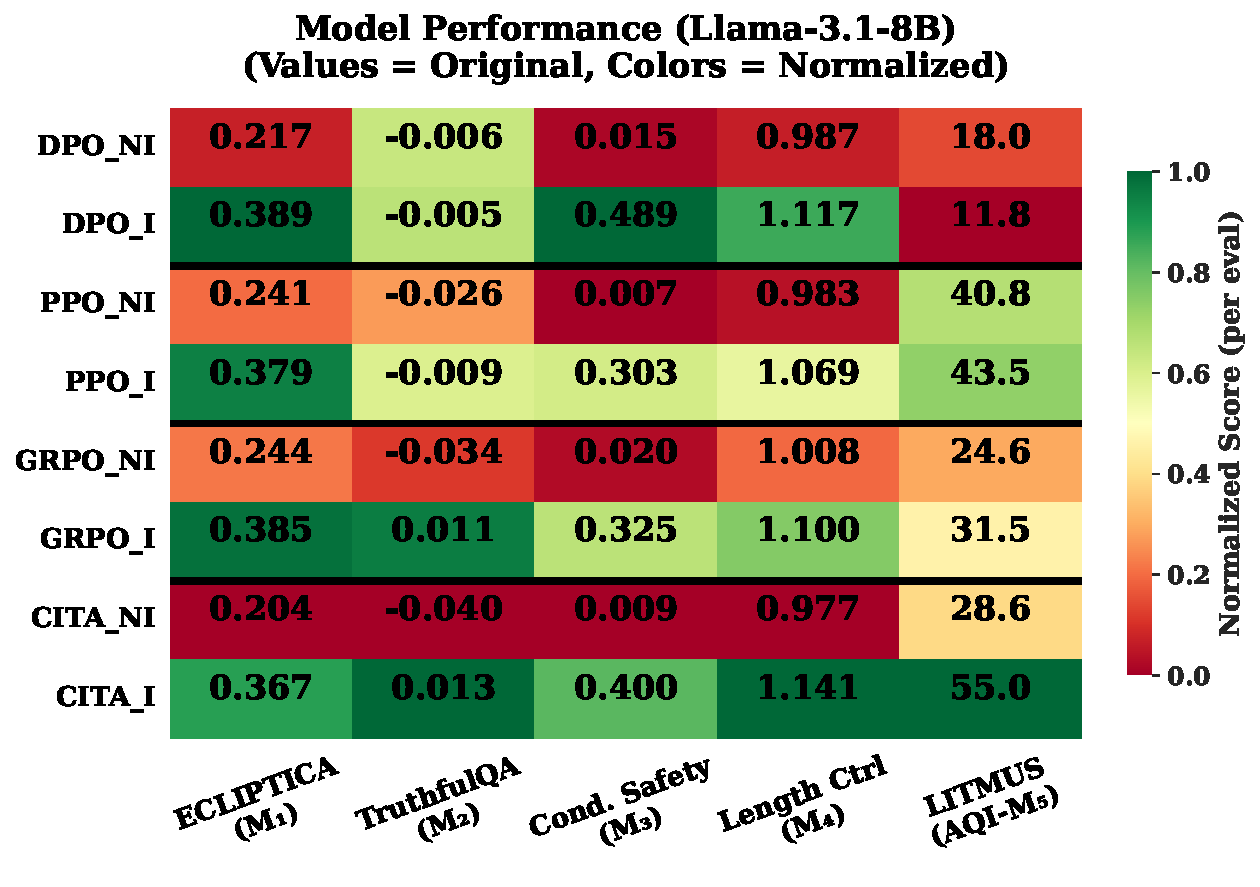
\includegraphics[width=\columnwidth]{figures/evaluation/combined_plots/heatmap_no_ci.pdf}
\vspace{-2em}
\caption{\textbf{Performance heatmap across 5 benchmarks.} Original scores with column-normalized colors (green = best, red = worst per column). NI = NoInstruct, I = Instruct. \textsc{CITA\_I} achieves highest AQI (55.0) and competitive performance across all metrics.}
\label{fig:heatmap_results}
\vspace{-1.5em}
\end{figure}

\vspace{-2mm}
\subsection*{Instruction Sensitivity: CITA vs.\ DPO}
\label{sec:improvement_comparison}

\noindent\textbf{Primary controlled comparison.} Instruction sensitivity measures how much a method \emph{moves} when we add behavioral instructions: $\Delta = \text{Instruct} - \text{NoInstruct}$. This isolates switching behavior from base capability.

\textbf{Comparison Design.} By evaluating NoInstruct vs. Instruct variants, we measure each method's \textit{instruction sensitivity}---the improvement from adding alignment instructions.


\begin{table}[H]
\centering
\footnotesize
\setlength{\tabcolsep}{4pt}
\renewcommand{\arraystretch}{1.2}
\begin{tabular}{@{}lcccc@{}}
\toprule
\textbf{Benchmark} & \textbf{DPO$\Delta$} & \textbf{PPO$\Delta$} & \textbf{GRPO$\Delta$} & \textbf{CITA$\Delta$} \\
\midrule
ECLIPTICA & \textbf{+0.172} & +0.138 & +0.141 & +0.162 \\ \hline
Truthful-QA & +0.001 & +0.017 & +0.045 & \textbf{+0.054} \\ \hline
Cond.\ Saf. & \textbf{+0.475} & +0.295 & +0.304 & +0.391 \\ \hline
Len.\ Ctrl & +0.130 & +0.086 & +0.092 & \textbf{+0.164} \\ \hline
AQI & $-$6.2 & +2.7 & +6.9 & \textbf{+26.4} \\
\bottomrule
\end{tabular}
\vspace{-1mm}
\caption{\textbf{Instruction sensitivity} ($\Delta=$ Instruct $-$ NoInstruct). \textsc{CITA} shows the strongest gains on TruthfulQA, Length Control, and AQI, while \textsc{DPO} leads on ECLIPTICA and Conditional Safety.}
\label{tab:improvement_comparison}
\vspace{-4mm}
\end{table}



\begin{comment}
    
\begin{table}[H]
\centering
\footnotesize
\setlength{\tabcolsep}{8pt}
\renewcommand{\arraystretch}{1.2}
\begin{tabular}{@{}clc@{}}
\toprule
\textbf{Rank} & \textbf{Method} & \textbf{Avg Radius} \\
\midrule
\#1 & \textbf{CITA} & \textbf{86.7\%} \\ \hline
\#2 & DPO & 56.1\% \\ \hline
\#3 & GRPO & 36.1\% \\ \hline
\#4 & PPO & 20.4\% \\
\bottomrule
\end{tabular}
\caption{\textbf{Ranking by average radius} (higher = better instruction alignment). \textbf{Overall instruction-alignment efficiency}: \textbf{CITA 86.7\%} vs DPO 56.1\% (+30.6 pp), GRPO 36.1\% (+50.6 pp), PPO 20.4\% (+66.3 pp).}
\label{tab:ranking_avg_radius}
\vspace{-4mm}
\end{table}
\end{comment}


\noindent\textbf{Takeaway \& Interpretation.} \textsc{CITA} delivers consistently strong \emph{instruction sensitivity} on \emph{controlled-switching} metrics—truthfulness-under-uncertainty separation, explicit length control, and axiom-level clustering—supporting the claim that it preserves distinct instruction-conditioned behavioral regimes within a shared backbone; moreover, at comparable accuracy it achieves larger margins than \textsc{DPO}, indicating sharper preference separation without sacrificing classification performance, a pattern \emph{consistent with} mandatory KL anchoring stabilizing instruction-conditioned updates.








% \vspace{-1mm}
% \section{Conclusion}
% \label{sec:conclusion}

% We introduced \textbf{CITA (Contrastive Instruction-Tuned Alignment)}, a framework for \textbf{instruction-aware alignment} where a single model can \textbf{switch behavioral regimes at inference time} via natural-language instructions. In contrast to static weight-encoded alignment (e.g., DPO~\cite{rafailov2023direct}, RLHF~\cite{ouyang2022training}), \textsc{CITA} targets \emph{stable, instruction-conditioned} policies under a shared backbone.

% \vspace{-2mm}
% \subsection{Key Findings}
% \label{sec:key_findings}

% \begin{enumerate}[leftmargin=*,itemsep=1pt]
%     \item \textbf{Strongest overall instruction alignment.} By the normalized radar-area efficiency metric (\cref{eq:efficiency}), \textsc{CITA} reaches \textbf{86.7\%}, exceeding \textsc{DPO} (56.1\%), \textsc{GRPO} (36.1\%), and \textsc{PPO} (20.4\%).
%     \item \textbf{Better directional switching where calibration matters.} On TruthfulQA, \textsc{CITA} shows a clear instruction-induced shift (\textbf{+0.054}) whereas \textsc{DPO} is nearly insensitive (\textbf{+0.001}).
%     \item \textbf{KL anchoring is a structural requirement.} In \textsc{CITA}, KL regularization is \textbf{mandatory} to maintain stable instruction-conditioned updates and avoid collapse under frequent switches.
%     \item \textbf{Beyond surface compliance.} On ISD, \textsc{CITA} improves policy-level alignment under fixed prompts, separating \emph{behavioral switching} from mere stylistic instruction-following.
% \end{enumerate}







\vspace{-1mm}
\section{Conclusion}
\label{sec:conclusion}

We presented \textbf{CITA (Contrastive Instruction-Tuned Alignment)}, a method for \textbf{instruction-aware alignment} that enables a single language model to \textbf{reliably switch behavioral regimes at inference time} using natural-language alignment instructions. Unlike static alignment approaches that encode a single policy into model weights (e.g., DPO~\cite{rafailov2023direct}, RLHF~\cite{ouyang2022training}), \textsc{CITA} learns a \emph{family of instruction-conditioned policies} under a shared backbone, stabilized by a mandatory KL trust region. Empirically, \textsc{CITA} achieves \textbf{86.7\%} overall instruction-alignment efficiency and exhibits correct directional adaptation on calibration-sensitive benchmarks such as TruthfulQA, where prior preference-optimization methods show little instruction sensitivity.

More broadly, this work reframes alignment as a \emph{runtime-controllable interface} rather than a training-time artifact. Instruction-conditioned alignment enables a single deployed model to serve multiple roles and policy contexts without retraining or maintaining separate checkpoints, while preserving stable and auditable behavior under switching.

% =============================================================================
% NOTE: Sections 7.1-7.3 (Benchmark-Specific Analysis, Combined Analysis, Key Insights)
% moved to separate file: 12_extended_results.tex (included in Appendix)
% See Appendix \ref{sec:appendix_extended_results} for detailed benchmark analysis
% =============================================================================



% \begin{table}[H]
% \centering
% \footnotesize
% \begin{tabularx}{\columnwidth}{@{}lXX@{}}
% \toprule
% \textbf{Benchmark} & \textbf{Cases} & \textbf{Instr. Types} \\
% \midrule
% ISD (ours) & 3,000 & 10 types \\
% TruthfulQA & 1,634 & HON/CONF \\
% Cond. Safety & 1,000 & STRICT/PERMIS. \\
% Length Control & 1,000 & CONC./DETAIL. \\
% AQI & 2,800 & 7 axioms \\
% \bottomrule
% \end{tabularx}
% \caption{Evaluation benchmarks. All use deterministic metrics.}
% \label{tab:benchmarks}
% \vspace{-4mm}
% \end{table}

% \paragraph{Metrics.}

% \begin{table}[H]
% \centering
% \footnotesize
% \begin{tabular}{@{}ll@{}}
% \toprule
% \textbf{Benchmark} & \textbf{Metric (Ideal Value)} \\
% \midrule
% ISD & Fidelity $\times$ Behavioral Shift (1.0) \\
% TruthfulQA & HON $-$ CONF uncertainty difference (+) \\
% Conditional Safety & $|$STRICT $-$ PERMISSIVE$|$ (1.0) \\
% Length Control & DETAILED/CONCISE word ratio ($>$4) \\
% AQI & (CHI + XB) / 2 clustering score (100) \\
% \bottomrule
% \end{tabular}
% \caption{Metric definitions. Higher is better for all except TruthfulQA (positive direction matters).}
% \label{tab:metrics}
% \vspace{-4mm}
% \end{table}

% \textbf{ISD Types}: Neutral, Conservative, Liberal, Regulatory, Empathetic, Safety, Educational, Concise, Professional, Creative.

% \textbf{AQI Axioms}: Civility, Duty, Empathy, Information, Justice, Well-being, Wisdom.



% stronger preference differentiation.





% =============================================================================
% NOTE: Sections 7.1-7.3 (Benchmark-Specific Analysis, Combined Analysis, Key Insights)
% moved to separate file: 12_extended_results.tex (included in Appendix)
% See Appendix \ref{sec:appendix_extended_results} for detailed benchmark analysis
% =============================================================================
